\section*{\large{INTRODUCCIÓN}}
\vspace{-0.25cm}
\justifying

\subsubsection*{\it{Sistema de conversión DC-DC}}
\vspace{-0.25cm}
Un sistema de conversión básico de conversión de potencia de CC a CC consta de una fuente de alimentación de CC, el convertidor CC-CC y una carga.
La fuente de CC provee una tensión de CC arbitraria al convertidor. El convertidor luego convierte el nivel del voltaje dado al valor requerido
por la carga, y lo suministra a la carga. La carga es un sistema de aplicación que opera con una tensión de CC fija y eventualmente consume potencia
eléctrica.

\begin{figure}[H]
    \centering
    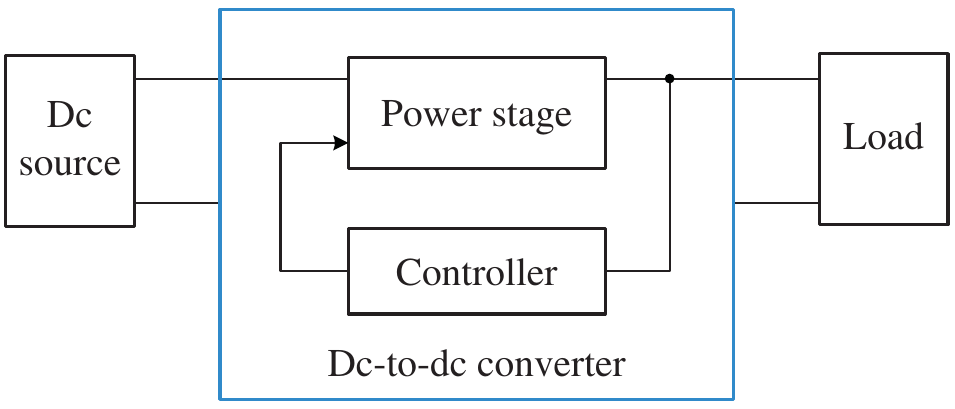
\includegraphics[height=4cm]{sistema_convertidor.png}
    \vspace{-0.25cm}
    \caption{Sistema autónomo de conversión de potencia de CC a CC.}
    \label{fig:sistema_convertidor}
\end{figure}
\vspace{-0.5cm}

La fuente de alimentación de CC no alcanza las características de una fuente de voltaje ideal en varios aspectos.
Primero, el nivel de voltaje de la fuente de CC podría variar con el tiempo, como es en el caso de las baterías, las celdas de combustible y otras
fuentes de CC independientes.

Segundo, una fuente de CA rectificada se utiliza frecuentemente como un sustituto de la fuente de CC. En este caso, la fuente de CA rectificada
usualmente contiene una cantidad considerable de componentes de CA, conocidas como ripple de CA. En adición, la salida de la fuente de CA rectificada
podría ser corrompida con varios ruidos.

Por esta razón, como se puede ver en la Figura \ref{fig:sistema_convertidor}, el convertidor está agrupado en dos bloques funcionales: la etapa de potencia
y el controlador. La etapa de potencia altera el nivel del voltaje de entrada al valor deseado utilizando varios componentes circuitales activos y pasivos,
mientras que el controlador provee las señales necesarias para que la etapa de potencia ejecute su función.

\subsubsection*{\it{El convertidor Buck ideal}}
\vspace{-0.25cm}
El convertidor Buck es la configuración de circuito más sencilla que realiza la conversión de potencia de CC a CC, reduciendo el voltaje.

\begin{figure}[H]
    \centering

    \begin{subfigure}[b]{\textwidth}
        \centering
        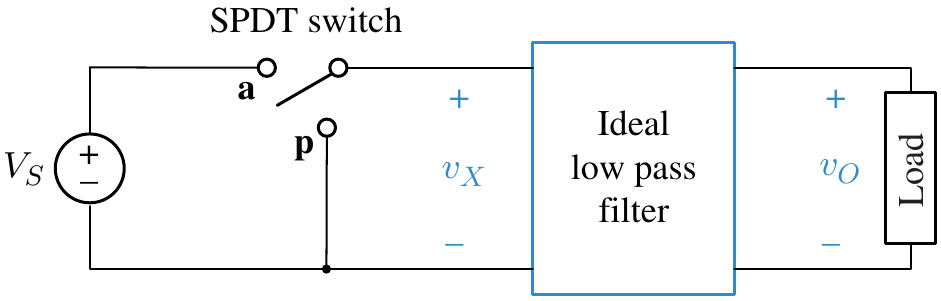
\includegraphics[height=3.5cm]{buck_ideal.png}
        \vspace{-0.25cm}
        \caption{Representación en diagrama de bloques.}
        \label{fig:buck_ideal_diagrama}
    \end{subfigure}
    \begin{subfigure}[b]{\textwidth}
        \centering
        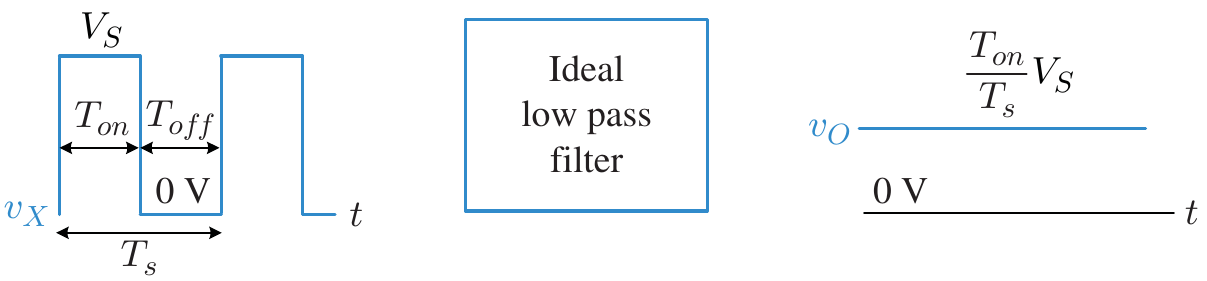
\includegraphics[height=3.5cm]{buck_ideal_filtro.png}
        \vspace{-0.25cm}
        \caption{Descripción en el dominio del tiempo.}
        \label{fig:buck_ideal_filtro}
    \end{subfigure}

    \vspace{-0.25cm}
    \caption{Conversión de potencia DC-DC reductora de tensión ideal.}
    \label{fig:buck_ideal}
\end{figure}
\vspace{-0.5cm}

La conversión reductora de tensión se explica utilizando un diagrama conceptual, como se muestra en la Figura \ref{fig:buck_ideal_diagrama}, consistiendo
de dos bloques funcionales: un interruptor unipolar de dos posiciones (SPDT) y un filtro pasa-bajos ideal. Dentro de un período de conmutación $T_s$, el
interruptor mantiene la posición \textbf{a} por $T_{on}$ y la posición \textbf{b} por $T_{off}$. El período de tiempo $T_{on}$ es definido como el período de encendido,
mientras que $T_{off}$ es denotado el período de apagado. La relación entre $T_{on}$ y $T_s$ es definido como la relación de trabajo o el ciclo de trabajo $D$ del
interruptor SPDT.

El interruptor SPDT transforma la tensión de entrada $V_S$ en una onda rectangular $v_X$, como se muestra en la figura \ref{fig:buck_ideal_filtro}.
La onda rectangular $v_X$ es luego aplicada a la entrada del filtro pasa-bajos ideal. Si la frecuencia de corte del filtro ideal, $\omega_c$, es menor que la
frecuencia fundamental de $v_X$, todos los componentes harmónicos son completamente bloqueados y solo la componente de CC aparece en la salida del filtro pasa-bajos:
\begin{equation}
    v_{o} = {\overline{v}}_X(t) = \dfrac{T_{on}}{T_{s}} \cdot V_S = D \cdot V_S
    \label{eq:buck_ideal}
\end{equation}

Esta conversión de potencia DC-DC tiene las siguientes propiedades:
\begin{itemize}[noitemsep]
    \item El circuito provee una tensión de CC pura para la carga, debido a las características ideales del filtro pasa-bajos.
    \item La ganancia de tensión del circuito, la relación $v_o$ a $V_S$, es simplemente la relación de trabajo $D$ del interruptor SPDT. Por lo tanto, el voltaje de salida
    es ajustado controlando el ciclo de trabajo del interruptor.
    \item Porque $0 < D < 1$, la tensión de salida $v_o$ es siempre menor que la tensión de entrada $V_S$.
\end{itemize}

Por estas razones, el convertidor Buck ideal es un convertidor de potencia CC-CC reductor de tensión.

\subsubsection*{\it{El convertidor Buck práctico}}
\vspace{-0.25cm}
En la práctica, se implementa el convertidor Buck reemplazando el interruptor SPDT ideal por conmutadores semiconductores, como un transistor MOSFET y un diodo.
El conmutador MOSFET es encendido y apagado por la señal de compuerta $V_{GS}$, mientras que el estado del diodo es determinado por la condición del conmutador MOSFET.
Cuando el MOSFET está encendido, el diodo está apagado porque la tensión de entrada $V_S$ polariza inversamente la junción p-n. En cambio, cuando el MOSFET está apagado,
las corriente del inductor fuerza al diodo a conducir.

Un filtro de segundo orden LC es utilizado como un sustituto funcional para el filtro pasa-bajos ideal. El fitro LC, a pesar de sus características lejanas a lo idea, provee
un filtrado más que adecuado para la mayoría de aplicaciones.

\begin{figure}[H]
    \centering
    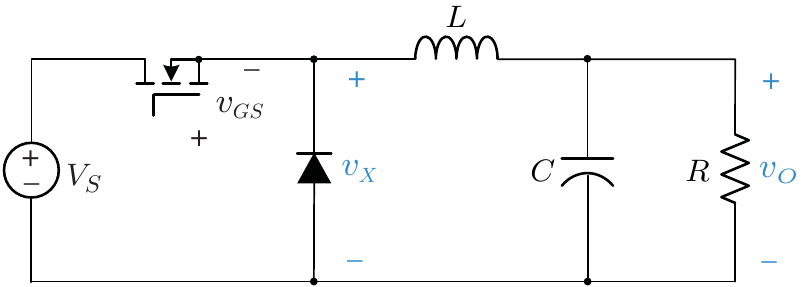
\includegraphics[height=4cm]{buck_generico.png}
    \vspace{-0.25cm}
    \caption{Convertidor Buck con par MOSFET-Diodo y filtro LC.}
    \label{fig:buck_practico}
\end{figure}
\vspace{-0.5cm}
\parencite{CHOI} % Ver donde habría que poner la cita